\chapter{Compute architecture and scheduling}
\begin{center}
    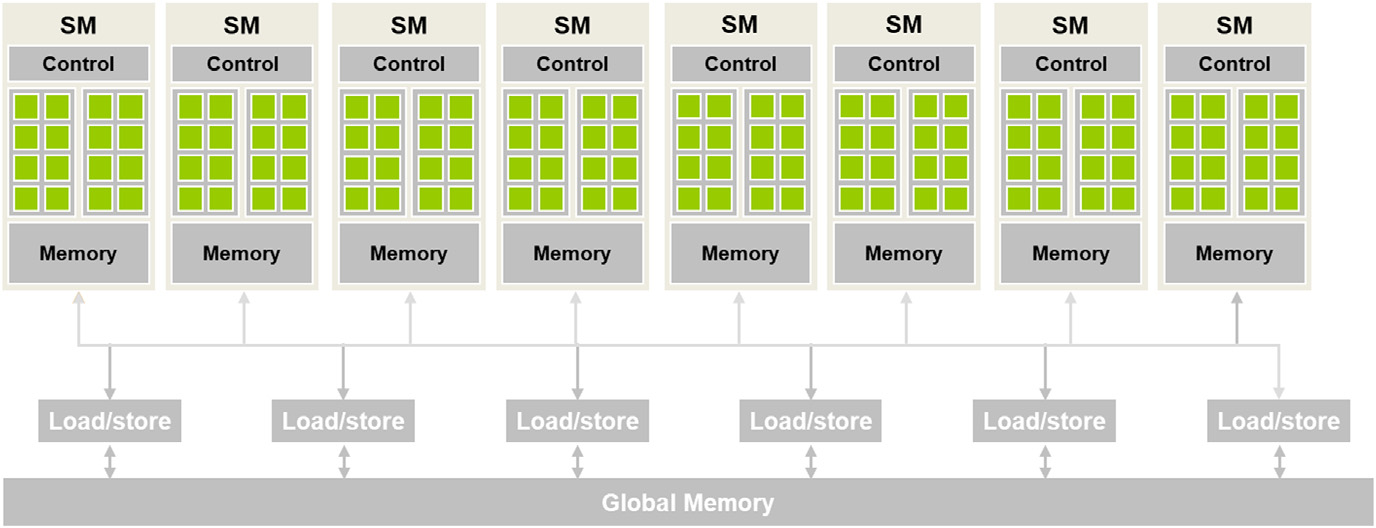
\includegraphics[width=0.7\linewidth]{Images/CompArch/CUDA_GPU.png}
\end{center}
\begin{itemize}
    \item A CUDA capable GPU is organized into an array of highly threaded streaming multiprocessors(SMs).
          \begin{itemize}
              \item Each SM $\rightarrow$ has several processing units called CUDA Cores (cores).
                    \begin{itemize}
                        \item Each Core $\rightarrow$ shares control logic and memory resources.
                    \end{itemize}
          \end{itemize}
\end{itemize}

\section{Block scheduling}
\begin{center}
    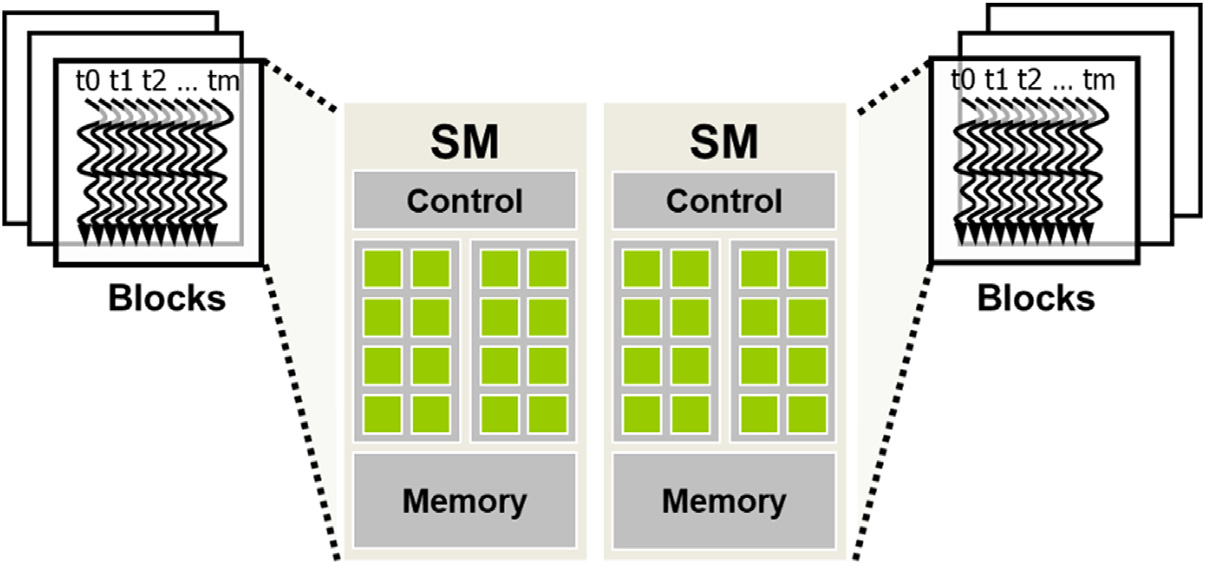
\includegraphics[width=0.7\linewidth]{Images/CompArch/block_assignment.png}
\end{center}
When the kernel is called, the CUDA runtime system launches a grid of threads that execute kernel code. The threads are attached to Streaming Multiprocessors (SMs) on a block-by-block basis.
\begin{itemize}
    \item i.e, \textbf{all the threads in a block are assigned to the same SM}.
    \item Multiple blocks are assigned to the same SM.
    \item \textbf{Blocks need to reserve hardware resources} to execute. $\implies$ A \textbf{limited number of blocks can be assigned to an SM.}
          \begin{itemize}
              \item As the \textbf{number of SMs} in a GPU is \textbf{limited}, the \textbf{total number of blocks that can be simultaneously executing on a CUDA device is limited}.
              \item Most grids contain many more blocks than this number. To ensure all the blocks in a grid get executed, the runtime system maintains a list of blocks that need to execute and assigns new blocks to SMs when previously assigned blocks complete execution.
          \end{itemize}
    \item This fashion of assignment of threads to SMs \textbf{guarantees that the threads in the same block are scheduled simultaneously on the same SM}. This \textbf{guarantee enables the threads in the same block to interact with each other} in ways that the threads across the blocks cannot.
\end{itemize}

\section{Synchronization and transparent scalability}